\chapter{L'utilizzo di Android per lo sviluppo del sensore Bluetooth}
\label{chap:app-separata}
Prima di sviluppare il sensore si è scelto di creare una piccola applicazione a sé stante con lo scopo di prendere dimestichezza con le librerie di Android per Java,
\begin{wrapfigure}[23]{r}{0.4\textwidth}
    \centering
    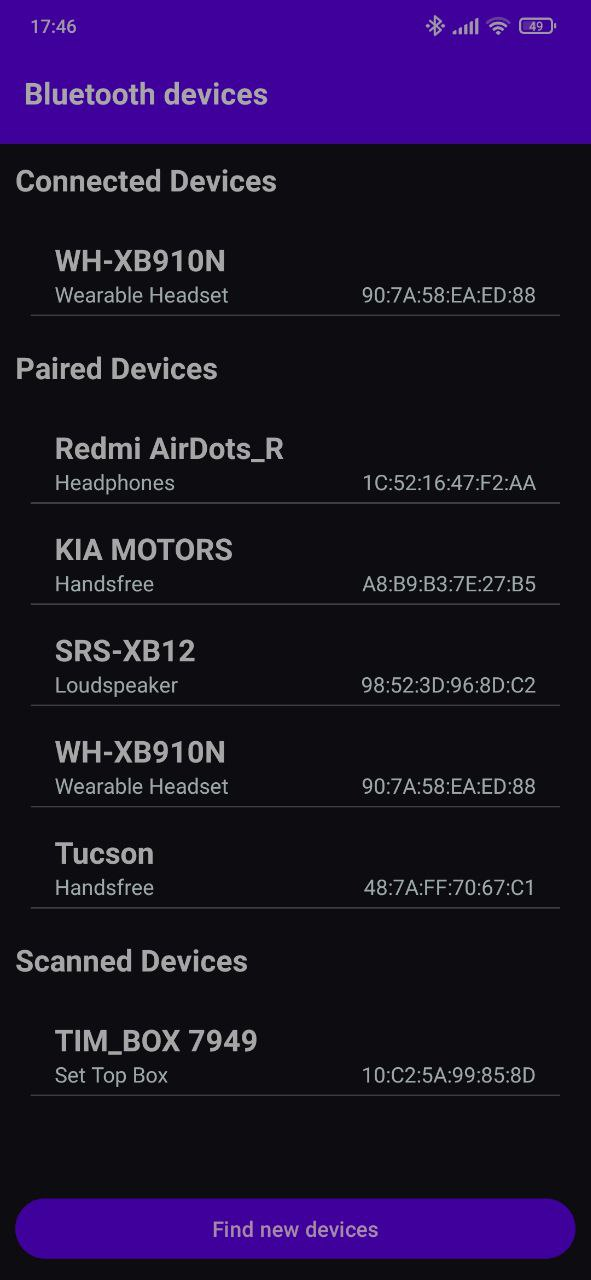
\includegraphics[width=0.9\linewidth]{images/separate_app.png}
    \caption{Interfaccia dell'applicazione}
    \label{fig:separate_app}
\end{wrapfigure}
 nello specifico con le sue funzionalità riguardanti la connettività via Bluetooth\cite{ref:bluetooth-doc}. Ciò è stato fatto al fine di trovare una strategia efficiente da adottare nello sviluppo del sensore finale in GeneroCity, dato che essa contiene molte altre funzionalità e di conseguenza sarebbe stato più difficoltoso effettuare questo tipo di sperimentazione al suo interno. Questa applicazione permette l'esecuzione di tre task, la cui implementazione è stata ritenuta un buon punto di partenza per lo sviluppo del sensore Bluetooth. Esse sono:
\begin{itemize}
    \item la rilevazione del cambiamento dello stato del modulo bluetooth dello smartphone, più specificatamente la sua accensione e lo spegnimento;
    \item l'ottenimento dei dati riguardanti i dispositivi che vengono connessi al Bluetooth;
    \item l'esecuzione di scansioni per trovare dispositivi nelle vicinanze.
\end{itemize}

In questo capitolo verranno quindi illustrati i vari componenti dell'applicazione e come essi implementano le suddette task consentendone la visualizzazione dei risultati. 

\section{I Broadcast Receiver}
Il primo problema che si è presentato nella realizzazione dell'applicazione è stato l'impossibilità di ottenere la lista dei dispositivi connessi al Bluetooth in maniera sincrona tramite le funzionalità messe a disposizione dalle API\footnote{Una API, acronimo di Application Software Interface, è un tipo di interfaccia software che permette ad un programma di offrire servizi e funzionalità ad altri software.} di Android. Infatti il sistema operativo non permette di essere interrogato direttamente dai singoli processi, piuttosto è esso a notificarli quando avvengono degli eventi di sistema, inviando dei messaggi denominati \textit{system broadcast}. Le applicazioni potranno quindi registrarsi per ricevere messaggi relativi ad eventi specifici, ad esempio quando avviene l'accensione e lo spegnimento della modalità aereo il sistema manderà un system broadcast a tutte le app registrate per ricevere questo evento. Questa registrazione avviene attraverso la creazione di oggetti la cui classe estende quella dei \textit{BroadcastReceiver}.\cite{ref:android-broadcast}

La classe sopracitata espone un metodo astratto, denominato \textit{onReceive}, il quale deve essere implementato per definire il comportamento adottato dal programma quando viene ricevuto un system broadcast. Questo metodo ha come parametri il contesto, vale a dire lo stato dell'applicazione al momento in cui è avvenuto, l'evento e l'intent, ossia una rappresentazione dell'evento che ha scaturito la notifica.

\begin{minted}[
framesep=2mm,
linenos,
bgcolor=LightGray,
breaklines
]{java}
public abstract void onReceive(Context context, Intent intent);
\end{minted}

Infine è necessario utilizzare il metodo registerReceiver della classe Context per attuare l'effettiva registrazione al fine di ricevere system broadcast e gestirli attraverso il broadcast receiver passato come parametro. Per far ciò bisogna inoltre dichiarare quali tipologie di eventi esso ascolta, creando un IntentFilter. Viene riportato qui sotto un esempio di codice dove viene registrato un broadcast receiver:
\begin{minted}[
framesep=2mm,
linenos,
bgcolor=LightGray,
breaklines
]{java}
BroadcastReceiver br = new MyBroadcastReceiver();
IntentFilter filter = new IntentFilter(APP_SPECIFIC_BROADCAST);
context.registerReceiver(br, filter);
\end{minted}

Tutti i broadcast receiver definiti si occuperanno solamente di catturare l'evento, sarà poi un metodo astratto, specifico per ognuno di essi, ad essere esteso per implementare l'algoritmo scaturito da esso. Questi metodi saranno estesi direttamente alla creazione dei receiver nella classe Controller, la quale verrà discussa nel paragrafo \ref{ref:controller}. Inoltre tutti i receiver intercettano gli eventi anche quando l'applicazione è in background, pertanto il funzionamento dell'app è inalterato quando essa è in esecuzione ma l'utente non la sta utilizzando direttamente. Di seguito verranno elencati i broadcast receiver implementati e, per ciascuno di essi, verranno discussi i system broadcast che riceveranno e riportato il codice del metodo \textit{onReceive}.

\subsection{Lo StatusChangeReceiver}
Esso è il broadcast receiver più semplice ed è stato definito per rilevare l'accensione e lo spegnimento del Bluetooth del dispositivo. Questo receiver si occuperà di intercettare gli eventi che cambiano lo stato della radio Bluetooth, ossia del tipo \textit{BluetoothAdapter.ACTION\_STATE\_CHANGED}.
\begin{minted}[
framesep=2mm,
linenos,
bgcolor=LightGray,
breaklines
]{java}
@Override
public void onReceive(Context context, Intent intent) {
    final String action = intent.getAction();

    if (action != null && action.equals(BluetoothAdapter.ACTION_STATE_CHANGED)) {
        final int state = intent.getIntExtra(BluetoothAdapter.EXTRA_STATE, BluetoothAdapter.ERROR);
        switch (state) {
            case BluetoothAdapter.STATE_OFF:
                onStatusChange(context, false);
                break;
            case BluetoothAdapter.STATE_TURNING_OFF:
                Toast.makeText(context, "Turning bluetooth off...", Toast.LENGTH_SHORT).show();
                break;
            case BluetoothAdapter.STATE_ON:
                onStatusChange(context, true);
                break;
            case BluetoothAdapter.STATE_TURNING_ON:
                Toast.makeText(context, "Turning bluetooth on...", Toast.LENGTH_SHORT).show();
                break;
            default:
                break;
        }
    }
}
\end{minted}

Nel caso in cui il Bluetooth sia stato acceso o spento verrà chiamato il metodo astratto \textit{onStatusChanged}, il quale ha come parametro un booleano che indica lo stato del Bluetooth (true quando è accesso e false se spento). Questo metodo sarà quindi esteso per definire cosa l'applicazione dovrà fare quando ciò avviene.
\begin{minted}[
framesep=2mm,
linenos,
bgcolor=LightGray,
breaklines
]{java}
public abstract void onStatusChange(Context context, boolean bluetoothStatus);
\end{minted}

\subsection{Il FoundDeviceReceiver}
Questo broadcast receiver si occupa di ricevere l'evento riguardante la scoperta di un nuovo dispositivo Bluetooth quando viene effettuata la scansione dei dispositivi nelle vicinanze. Esso verrà notificato degli eventi di tipo \textit{BluetoothDevice.ACTION\_FOUND} e si occuperà di prelevare le informazioni dei dispositivi rilevati attraverso la funzione di utilità \textit{BluetoothDeviceUtils.map}. Essa prende in input il dispositivo Bluetooth e restituisce un oggetto che e ne contiene le informazioni di interesse per l'applicazione (indirizzo MAC, nome del dispositivo e classe bluetooth).
\begin{minted}[
framesep=2mm,
linenos,
bgcolor=LightGray,
breaklines
]{java}
@Override
public void onReceive(Context context, Intent intent) {
    String action = intent.getAction();

    if (action == null 
            || !action.equals(
            android.bluetooth.BluetoothDevice.ACTION_FOUND
        )) {
        return;
    }
    
    android.bluetooth.BluetoothDevice device;
    if (Build.VERSION.SDK_INT >= Build.VERSION_CODES.TIRAMISU) {
        device = intent.getParcelableExtra(
                android.bluetooth.BluetoothDevice.EXTRA_DEVICE,
                android.bluetooth.BluetoothDevice.class
        );
    } else {
        device = intent.getParcelableExtra(
                android.bluetooth.BluetoothDevice.EXTRA_DEVICE
        );
    }
    if (device == null) {
        return;
    }
    
    BluetoothDevice newDevice = BluetoothDeviceUtils.map(device);
    onDeviceFound(newDevice);
}
\end{minted}

Come si può vedere dal codice una volta ottenuti i dati del dispositivo viene chiamato un metodo astratto denominato \textit{onDeviceFound} che verrà esteso per salvare il dispositivo in una struttura dati.
\begin{minted}[
framesep=2mm,
linenos,
bgcolor=LightGray,
breaklines
]{java}
public abstract void onDeviceFound(BluetoothDevice device);
\end{minted}


\subsection{Il ConnectionReceiver}
Gli eventi di tipo \textit{BluetoothDevice.ACTION\_ACL\_CONNECTED} e \textit{BluetoothDevice.ACTION\_ACL\_DISCONNECTED} per ottenere informazioni sui dispositivi che vengono connessi e disconnessi dal Bluetooth saranno gestiti da questo receiver. Quando ciò avviene verrà utilizzata la funzione di mappatura citata precedentemente per prelevarne le informazioni di interesse dai dispositivi.
\begin{minted}[
framesep=2mm,
linenos,
bgcolor=LightGray,
breaklines
]{java}
@Override
public void onReceive(Context context, Intent intent) {
    String action = intent.getAction();

    if (action == null 
        || !action.equals(
            android.bluetooth.BluetoothDevice.ACTION_ACL_CONNECTED
        ) && !action.equals(
            android.bluetooth.BluetoothDevice
                .ACTION_ACL_DISCONNECTED
        )) {
        return;
    }

    android.bluetooth.BluetoothDevice device;
    if (Build.VERSION.SDK_INT >= Build.VERSION_CODES.TIRAMISU) {
        device = intent.getParcelableExtra(
                android.bluetooth.BluetoothDevice.EXTRA_DEVICE,
                android.bluetooth.BluetoothDevice.class
        );
    } else {
        device = intent.getParcelableExtra(
                android.bluetooth.BluetoothDevice.EXTRA_DEVICE
        );
    }

    if (device == null) {
        return;
    }

    BluetoothDevice newDevice = BluetoothDeviceUtils.map(device);

    if (action.equals(android.BluetoothDevice.ACTION_ACL_CONNECTED)) {
        onDeviceConnection(context, newDevice);
    } else {
        onDeviceDisconnection(context, newDevice);
    }
}
\end{minted}

Infine verrà chiamato il metodo astratto \textit{onDeviceConnection} in caso di connessione del dispositivo oppure \textit{onDeviceDisconnection} se si tratta di una disconnessione. Questi metodi verranno estesi per tenere aggiornata una struttura dati che mantiene in memoria i dispositivi connessi via Bluetooth.
\begin{minted}[
framesep=2mm,
linenos,
bgcolor=LightGray,
breaklines
]{java}
public abstract void onDeviceConnection(Context context, BluetoothDevice device);
public abstract void onDeviceDisconnection(Context context, BluetoothDevice device);
\end{minted}

\subsection{L'ImplicitConnectionReceiver}
La creazione di questo receiver deriva dal fatto che tutti quelli descritti precedentemente vengono registrati una volta che viene avviata l'applicazione, pertanto se ci sono già connessi dei dispositivi Bluetooth prima dell'avvio il ConnectionReceiver non è in grado di rilevarli. L'ImplicitConnectionReceiver nasce per risolvere questo problema, difatti esso è una sottoclasse di ConnectionReceiver e funzionerà anche quando l'applicazione è completamente chiusa: esso viene registrato nel manifest\footnote{Il manifest Android è un file che definisce la struttura, le funzionalità e i requisiti di un'applicazione Android.} dell'applicazione e sarà quindi il sistema operativo a "svegliarla" se essa non è in esecuzione, così da permettere l'esecuzione di codice in risposta ad una connessione o disconnessione di un dispositivo Bluetooth. Segue la porzione di manifest dove viene dichiarato il receiver specificandone gli intent per cui esso sarà notificato.
\begin{minted}[
framesep=2mm,
linenos,
bgcolor=LightGray,
breaklines
]{xml}
<receiver 
    android:name="receivers.ImplicitConnectionReceiver"
    android:exported="true">
    <intent-filter>
        <action 
            android:name= "android.bluetooth.device.action.ACL_CONNECTED"/>
        <action
            android:name= "android.bluetooth.device.action.ACL_DISCONNECTED"/>
    </intent-filter>
</receiver>
\end{minted}

Esso essendo di tipo ConnectionReceiver eredita anche il metodo onReceive di quest'ultimo, tuttavia deve fornire un implementazione dei suoi metodi astratti. Nel caso della connessione di un dispositivo il metodo \textit{onDeviceConnection} si occuperà di caricare un'insieme dei dispositivi connessi in quel momento da un file, aggiungere il dispositivo connesso in quel momento e salvare l'insieme aggiornato sul file.
\begin{minted}[
framesep=2mm,
linenos,
bgcolor=LightGray,
breaklines
]{java}
@Override
public void onDeviceConnection(Context context, BluetoothDevice device) {
    Set<BluetoothDevice> connectedDevices = loadConnectedDevices(context);
    connectedDevices.add(device);
    saveConnectedDevices(context, connectedDevices);
}
\end{minted}

Per quando riguarda il metodo \textit{onDeviceDisconnection} viene fatta pressoché la medesima cosa: viene caricato l'insieme dei dispositivi, rimosso il dispositivo disconnesso e salvato l'insieme aggiornato.
\begin{minted}[
framesep=2mm,
linenos,
bgcolor=LightGray,
breaklines
]{java}
@Override
public void onDeviceDisconnection(Context context, BluetoothDevice device) {
    Set<BluetoothDevice> connectedDevices = loadConnectedDevices(context);
    connectedDevices.remove(device);
    saveConnectedDevices(context, connectedDevices);
}
\end{minted}

Grazie a questo receiver il Controller, non appena verrà istanziato all'avvio dell'applicazione, potrà ottenere i dispositivi connessi precedentemente l'avvio in quanto verranno caricati dal file da esso aggiornato.

\section{Il Controller} \label{ref:controller}
Il Controller è l'unità centrale dell'applicazione infatti esso si occupa di mantenere gli insiemi dei dispositivi Bluetooth accoppiati al telefono\footnote{Con accoppiamento Bluetooth si intende il pairing, ossia il processo in cui due dispositivi Bluetooth effettuano la prima connessione e si scambiano le chiavi di sicurezza, le quali verranno memorizzate per permettere di effettuare rapidamente le connessioni successive.}, quelli rilevati dalle scansioni e infine i dispositivi connessi. Esso implementa due design pattern\footnote{Un design pattern, traducibile in schema di progettazione, nell'ambito dell'ingegneria del software è una soluzione generale ad un problema ricorrente.}: il \textbf{singleton pattern}, il quale consente alla classe Controller di avere un'unica istanza accessibile da qualunque punto del codice, e l'\textbf{observer pattern} che permette ad a altri oggetti di registrarsi per venire notificati dal Controller quando esso cambia il suo stato. In particolare lo stato del Controller è rappresentato da i suoi seguenti attributi:
\begin{itemize}
    \item \textit{isBluetoothEnabled}, un flag che indica se il modulo Bluetooth del dispositivo è acceso o spento;
    \item \textit{pairedDevices}, l'insieme dei dispositivi Bluetooth accoppiati allo smartphone;
    \item \textit{scannedDevices}, l'insieme dei dispositivi Bluetooth trovati durante l'ultima scansione;
    \item \textit{connectedDevices}, l'insieme dei dispositivi Bluetooth connessi allo smartphone.
\end{itemize}

Inoltre è presente una lista di listener, ossia degli oggetti che verranno notificati dal Controller ogni qualvolta esso cambierà stato. Nello specifico si tratta di una lista di \textit{Runnable}, ossia un'interfaccia funzionale\footnote{In Java un'interfaccia funzionale è un'interfaccia che contiene un solo metodo astratto. Esse permettono di utilizzare il paradigma di programmazione funzionale, facendo in modo di rappresentare delle funzioni come oggetti e potendole quindi passare come parametri ad altre funzioni.} il cui metodo non prende input né produce output ma esegue semplicemente una sequenza di istruzioni. Essi verranno eseguiti sequenzialmente uno dopo l'altro ogni volta che verrà chiamato il metodo \textit{notifyListener}, cosa che avverrà ad ogni cambiamento di stato del Controller.

Come detto in precedenza il Controller utilizza i broadcast receiver sopra descritti in modo da poter aggiornare il suo stato in risposta agli eventi di sistema. Tutti i receiver verranno creati come costanti della classe Controller e saranno registrati nel suo costruttore. Nello specifico vengono estese in maniera anonima le loro classi in modo da fornire un'implementazione dei metodi astratti. Di seguito verrà descritto come gli aggiornamenti di stato avvengono attraverso questi metodi.

\subsection{Stato del modulo Bluetooth (accensione e spegnimento)}
Per rilevare l'accensione e lo spegnimento del Bluetooth dello smartphone il Controller crea uno StatusChangeReceiver fornendo un'implementazione del metodo onStatusChange. Esso ha il compito di assegnare il nuovo valore al flag isBluetoothEnabled del controller sulla base del parametro booleano bluetoothStatus, il quale sarà true se il bluetooth è acceso o false altrimenti. In caso di spegnimento, verrà svuotato l'insieme dei dispositivi connessi. Infine verranno notificati i listener del cambiamento.
\begin{minted}[
framesep=2mm,
linenos,
bgcolor=LightGray,
breaklines
]{java}
private final StatusChangeReceiver statusChangeReceiver = new StatusChangeReceiver() {

        @Override
        public void onStatusChange(Context context, boolean bluetoothStatus) {
            isBluetoothEnabled = bluetoothStatus;
            if (!bluetoothStatus) {
                connectedDevices.clear();
            }
            notifyListeners();
        }
};
\end{minted}

\subsection{Connessione e disconnessione di un dispositivo}
Allo stesso modo verrà creato un ConnectionReceiver per aggiornare l'insieme dei dispositivi connessi quando uno di essi si connette o disconnette. Vengono quindi implementati i metodi onDeviceConnection e onDeviceDisconnection per far ciò: nel primo viene aggiunto il dispositivo ottenuto all'insieme dei dispositivi connessi mentre nel secondo il dispositivo viene rimosso. In entrambi i casi vengono notificati i listener.
\begin{minted}[
framesep=2mm,
linenos,
bgcolor=LightGray,
breaklines
]{java}
private final ConnectionReceiver connectionReceiver = new ConnectionReceiver() {

    @Override
    public void onDeviceConnection(Context context, BluetoothDevice device) {
        connectedDevices.add(device);
        notifyListeners();
    }

    @Override
    public void onDeviceDisconnection(Context context, BluetoothDevice device) {
        connectedDevices.remove(device);
        notifyListeners();
    }
};
\end{minted}

\subsection{Scoperta di un nuovo dispositivo durante la scansione}
Quando invece verrà effettuata la scansione dei dispositivi Bluetooth nelle vicinanze sarà il FoundDeviceReceiver a essere notificato ogni volta che ne viene trovato uno. Viene infatti implementato il suo metodo onDeviceFound per aggiungere il dispositivo all'insieme dei dispositivi trovati tramite la scansione e successivamente vengono notificati i listener del controller.
\begin{minted}[
framesep=2mm,
linenos,
bgcolor=LightGray,
breaklines
]{java}
private FoundDeviceReceiver foundDeviceReceiver = new FoundDeviceReceiver() {

    @Override
    public void onDeviceFound(BluetoothDevice device) {
        scannedDevices.add(newDevice);
        notifyListeners();
    }
};
\end{minted}

\section{La presentazione dei dati}\label{ref:presentation}
L'ultimo componente di quest'applicazione è l'interfaccia utente che permetterà la visualizzazione dispositivi amministrati dal Controller e di far partire le scansioni Bluetooth attraverso un bottone. Essa mostrerà i dispositivi divisi in tre elenchi differenti: uno per i dispositivi connessi, uno per quelli accoppiati e infine uno per quelli trovati via scansione. Queste liste sono amministrate da tre oggetti diversi tutti appartenenti alla classe \textit{BluetoothDeviceAdapter}, la quale si occupa di convertire gli elementi di una lista di dispositivi in una componente grafica che ne riporta le relative informazioni, come visibile in figura \ref{fig:separate_app}.
Inoltre in questa classe è presente un metodo astratto, denominato \textit{updateDevices}, che si occupa di aggiornare la lista dei dispositivi dell'adapter:
\begin{minted}[
framesep=2mm,
linenos,
bgcolor=LightGray,
breaklines
]{java}
public abstract void updateDevices();
\end{minted}
Esso sarà implementato alla creazione dei vari BluetoothDeviceAdapter in modo da ottenere dal Controller la lista dei dispositivi utili per l'adapter e successivamente notificarlo del cambiamento, così facendo esso renderizzerà nuovamente i suoi componenti grafici con i nuovi dati. Poiché l'implementazione è pressoché uguale per tutti gli adapter, si riporta come esempio solamente il codice di quello utilizzato per aggiornare i dispositivi connessi:
\begin{minted}[
framesep=2mm,
linenos,
bgcolor=LightGray,
breaklines
]{java}
BluetoothDeviceAdapter connectedDeviceAdapter = new BluetoothDeviceAdapter(this) {
    @Override
    public void updateDevices() {
        BluetoothController controller = BluetoothController
            .getInstance(MainActivity.this);
        devices = controller.getConnectedDevices();
        notifyDataSetChanged();
    }
};
\end{minted}
L'unica differenza che avranno gli altri BluetoothDevice adapter è quale lista di dispositivi essi richiederanno al Controller: per ottenere la lista aggiornata l'adapter che si occupa dei dispositivi accoppiati userà il metodo \textit{getPairedDevices} del Controller, quello che si occupa dei dispositivi scansionati \textit{getScannedDevices}, mentre, come visto sopra, quello relativo ai dispositivi connessi \textit{getConnectedDevices}.

Infine i metodi updateDevices di ogni BluetoothDeviceAdapter saranno registrati come listener del Controller. In tal modo ogni qual volta viene aggiornato lo stato di quest'ultimo e verranno notificati i listener questi metodi saranno eseguiti così da avere un riscontro grafico dell'aggiornamento avvenuto.
\begin{minted}[
framesep=2mm,
linenos,
bgcolor=LightGray,
breaklines
]{java}
controller.addListener(pairedDeviceAdapter::updateDevices);
controller.addListener(scannedDeviceAdapter::updateDevices);
controller.addListener(connectedDeviceAdapter::updateDevices);
\end{minted}

Ora che sono stati definiti tutti i componenti si può fornire un esempio del flusso di aggiornamento dell'applicazione, nello specifico esso verrà descritto in seguito alla connessione di un dispositivo Bluetooth: quando ciò accade il ConnectionReceiver viene notificato il quale esegue il metodo onDeviceConnection, che si occupa di aggiungere il dispositivo all'insieme dei dispositivi connessi del Controller. Una volta fatto ciò, a seguito del cambiamento di stato, verranno eseguiti sequenzialmente tutti i listener registrati. Tra di essi è presente il metodo updateDevices del connectedDeviceAdapter il quale interrogherà il Controller per ottenere la lista aggiornata dei dispositivi connessi e farà partire la procedura di rendering grafico della lista utilizzando i nuovi dati ottenuti. In maniera equivalente ciò avverrà per tutte le altre liste quando accade un evento che aggiorna uno degli insiemi dei dispositivi ed invece, per quanto riguarda il cambiamento di stato del modulo Bluetooth del telefono, se il Bluetooth viene spento le liste saranno rimpiazzate da un messaggio che intima l'utente di accenderlo e saranno nuovamente mostrate quando esso viene acceso. 

\section{Testing}
A pari passo con lo sviluppo di questa applicazione è stato verificato il suo funzionamento su più smartphone e, al termine di esso, è stato possibile rilevare le connessione di dispositivi Bluetooth, sia con l'applicazione in foreground che in background, ed effettuare scansioni per trovarne di nuovi, il tutto con successo e senza incorrere in nessun tipo di errore. Inoltre qualche test è stato effettuato utilizzando il Bluetooth di alcune autoradio ed è stato notato che tutte le macchine prese in esame sono rilevabili via scansione Bluetooth solamente quando viene effettuata la procedura per accoppiare un nuovo smartphone ad esse. Non poter trovare le macchine nelle vicinanze attraverso la scansione rende l'utilizzo di questa funzionalità pressoché inutile in GeneroCity, di conseguenza si è scelto di non implementarla nel sensore Bluetooth.
A questo punto si è potuto procedere con l'implementazione del sensore Bluetooth andando ad integrare in GeneroCity un sistema basato su quanto progettato per quest'applicazione

Nel prossimo capitolo verrà illustrata Generocity e in particolare il suo sistema di sensori per poi descrivere, nel capitolo \ref{chap:Bluetooth-sensor}, l'integrazione del nuovo sensore Bluetooth.